\documentclass[natbib,12pt]{article}

\usepackage[american]{babel}
\usepackage[utf8x]{inputenc}
\usepackage{amsmath}
\usepackage{graphicx}
\usepackage[colorinlistoftodos]{todonotes}
\usepackage{varioref}
\usepackage[hidelinks]{hyperref}
\usepackage[T1]{fontenc}

\title{CISC 610-90- O-2018/Late Fall Assignment 3}

\author{Youwei Lu}
\date{}

%\abstract{Referring to Operating Systems architecture, the topic of this assignment is on the ``Memory Management'' which is part of the computer's physical memory or Random-Access Memory (RAM) organization.}

\begin{document}
\maketitle
	
	\section{Runtime Performance of Merge Sort}
	\subsection{Random Data, in small and big set}
	Different test data is used to compare the runtime performance of merge sort. 
	
5 different numbers of random test data are compared, from small set (10) to big set (100000), and the runtime is recorded for each set. As the data is randomized, the runtime is different in each run. One batch test result is shown in Table.~\ref{tab:randomTest}.

	\begin{table}[htpb]
	\centering
	\begin{tabular}{l|l}
		Test Numbers & Runtime (ns) \\\hline
		10 & 8222 \\
		100 & 149420  \\
		1000 & 2850774 \\
		10000 & 96666016 \\
		100000 & 2771315573 
	\end{tabular}
	\caption{\label{tab:randomTest}Runtime for random test data.}
	\end{table}

To clearly compare the performance, the runtime results are shown in Figure~\ref{fig:mergesort}, along with the theoretical time complexity function $O(n\log n)$ ($\times 1000$ for better display) of merge sort. The blue curve shows the runtime measurement, and the red line shows the theoretical curve, versus data numbers. Although influenced by many other reasons, the runtime is majorly determined by time complexity, and the figure shows that the runtime curve is very close to the theoretical curve. 
	
\begin{figure}[htpb]
	\centering
	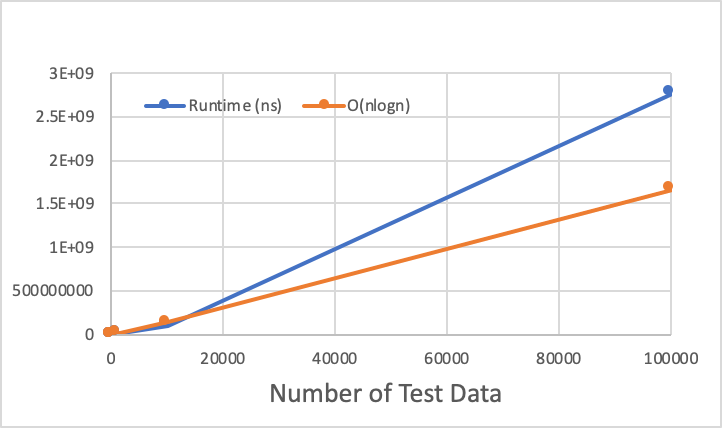
\includegraphics[width=1\linewidth]{merge_sort}
	\caption{Compare runtime performance for different numbers of data set}
	\label{fig:mergesort}
\end{figure}

\subsection{Other test data}
Now compare the test data with sorted set, partially sorted and sorted in opposite order, with the same numbers of data input, 100.
Following lists the data inputs:
\begin{itemize}
	\item Sorted: [1, 2, ...  99, 100]
	\item Partially sorted: [1, 2, ... , 24, 25, random, random, ... , random, random, 76, 77, ... , 99, 100]
	\item Sorted in opposite order: [100, 99, ... , 2, 1]
\end{itemize}

Again, due to random data and uncertainties of computer process, the runtime result is not the same every time, and one batch result is shown in Table.~\ref{tab:otherTest}.

	\begin{table}[htpb]
	\centering
	\begin{tabular}{l|r}
		Data types & Runtime (ns) \\\hline
		Sorted & 16649 \\
		Partially sorted & 23121  \\
		Sorted in opposite order & 14770 
	\end{tabular}
	\caption{\label{tab:otherTest}Runtime for sorted, partially sorted, and sorted in opposite order test data.}
\end{table}

It shows that all runtime results in for different types of data are in the same order of magnitude (including the 100 numbers of random data in Table.~\ref{tab:randomTest}), because for all kinds of data input, no matter best case, average case, or worse case, the time complexity of merge sort algorithm is $O(n\log n)$.

\section{BST}
\subsection{Time Complexity}
sumNodes traverses all nodes in BST, no more, no less, exactly each nodes one time (and add their values at the same time), thus the time complexity for sumNodes should be $O(n)$. 

The averageTree traverses all nodes two times, one for count the nodes, another for adding the total value, thus time complexity if $O(2n) = O(n)$.

\subsection{Space Complexity}
The space complexity of BST traverse depends on the depth of tree, that is, $O(\log n)$. sumNodes just need one more constant space for the sum, so the space complexity is $O(\log n + 1) = O(\log n)$. Similarly, averageTree simply need another constant space for the count, so its space complexity is $O(\log n + 2) = O(\log n)$. 

\end{document}

%
% Please see the package documentation for more information
% on the APA6 document class:
%
% http://www.ctan.org/pkg/apa6
%